% Source: Weinberg GR, physical PDF p. 340 (printed p. 318).
% Coverage: Figure 11.2, configurations of stellar equilibrium.
% Status: source plot extracted at source resolution; source-reviewed.
% Uncertainties: none.

\begingroup
\renewcommand{\thefigure}{11.2}
\begin{figure}[htbp]
  \centering
  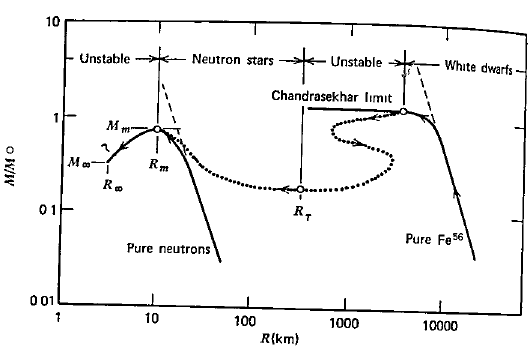
\includegraphics[width=0.83\textwidth]{figures/chapter11/fig11-02.png}
  \caption{Configurations of stellar equilibrium. The solid curves on the
  left and right represent the Oppenheimer--Volkoff%
  \hyperref[ch11-ref-10]{\textsuperscript{10}} solution for a pure neutron
  star and the Chandrasekhar%
  \hyperref[ch11-ref-8]{\textsuperscript{8}} solution for a pure
  \(\mathrm{Fe}^{56}\) white-dwarf star, respectively. The dashed lines give
  the extrapolated nonrelativistic solutions in these two cases. The dotted
  line represents the interpolating solution of Harrison, Thorne, Wakano, and
  Wheeler,\hyperref[ch11-ref-12]{\textsuperscript{12}} which takes into
  account the shift in chemical composition from \(\mathrm{Fe}^{56}\) to
  neutrons. Arrows indicate the direction of increasing central density. As
  shown in Theorem~1, the various transitions between stability and
  instability occur at the maxima and minima of \(M\), marked here with small
  circles.}
  \label{fig:11.2}
\end{figure}
\endgroup
